\pagebreak

\chapter{Zynq Communication Between the CPU and the FPGA}\label{ch:zynqcpu}

    The following assumes the use of a Linux kernel on the Zynq platform and a
    Linux, Unix or OSX operating system on a host computer for CPU code
    cross-compilation and execution of some of the support programs.
    
    This interface is very similar to the serial CPU interface described in the
    previous chapter (\autorefph{ch:serialcpu}). Much of the code is common to
    both.

    The board file xilinx/zynq\_axi.3pl includes source xilinx/cpu.3pl.
    Procedure create\_bus\_interfaces() in xilinx/zynq\_axi.3pl executes at the
    end of the main code to create the bus interface logic.

    GP bus 0 is used for reading 3PL expressions (i.e. value mode variables) or
    writing 3PL static or queue mode variables. GP bus 1 is used to read or
    write 3PL memory variables. Burst transfers of up to 8 32-bit words are
    supported. The four HP buses are used to implement 64-bit wide DMA transfers
    between the FPGA and CPU. Thus far the default 100MHz clock has been used
    for all buses. The CPU to FPGA interfaces are described in
    \autorefph{chap:lmzynqaxilib}.
    
    For this interface to operate the Zynq Linux device tree must provide
    entries for axi\_mgp0, axi\_mgp1 and axi\_hpbuf and must also provide
    interrupt events 0 to 15. An example is shown in
    \autorefph{ch:zynq_device_tree}.
    
    The following source code, prog.3pl, is an example of a simple 3PL program
    using CPU interfaces -
    
    \begin{lstlisting}[gobble=4, language=threepl]
        module "boards/avnet/microzed_7010.3pl"
        
        class(cpu, cpu_api());  // CPU API class

        static(a, "int:25");
        static(b, "int:18");

        cpu.write(a <- "A");    // write to {\bf a} from CPU
        cpu.write(b <- "B");    // write to {\bf a} from CPU

        static(p, "int:48");

        p <- a * b;

        cpu.read(p, "P");       // read from {\bf p} to CPU

        cpu.receive_event("INT", p == 1);   // interrupt when p == 1
    \end{lstlisting}
    
    Static variables {\bf a} and {\bf b} can be written to by the CPU. The
    product is assigned to p (in every clock cycle), which can be read by the
    CPU. The strings "A", "B" and "P" are names with which to refer to the
    interfaces within CPU code.
    
    Note that the interrupt {\bf INT} occurs when the expression
    {\bf p == 1} goes from false to true.
    
    When the program is compiled and executed by 3pl
    \autorefph{chap:run3pl}) the following files will be produced -
    \blist
    \item   {\bf prog.edif} - netlist file
    \item   {\bf prog.xdc} - Vivado constraints file
    \item   {\bf prog.bit} - configuration bit file
    \item   {\bf prog.info} - CPU/FPGA interface information (JSON) file
    \item   {\bf prog.rpt} - report file
    \item   {\bf prog.net} - optional list of net labels
    \blend
    The bit file is produced by a default post-processing module and can be
    supressed by specifying the -s option (skip) to 3PL. In that case the
    place-and-route can be performed by shell script edif2bit
    (sources/fpga\_platforms/edif2bit/edif2bit) or by the simple bash script
    run\_vivado (sources/fpga\_platforms/run\_vivado).
    
    The configuration file may be compressed using gzip
    
    The configuration file can be loaded into the FPGA manually by
    \verb'cat >/dev/xdevcfg'. Alternatively The configuration file or compressed
    configuration file can be converted into a byte array in CPU application
    code - see below.
    
    The CPU/FPGA interface information file prog.info is in JSON format and
    describes the CPU/FPGA interface.
     
    \begin{verbatim}
        {
            "version": {
                "major": 1,
                "minor": 0
            },
            "directives": {
                "ALU": "false",
                "FIFO": "false",
                "OS": "mac os x",
                "QUEUEREG": "false",
                "arch": "x86_64",
                "compileOnly": "false",
                "compilerMakeDate": "2022-04-04 14:45:06 +1000",
                "continuous": "false",
                "currentDirectory": "/Users/dun202/snark/src/test/zynq_int_test",
                "date": "2022-07-05 10:26:31 +1000",
                "designName": "prog",
                "family": "XC7",
                "filePath": "false",
                "forceExec": "true",
                "gatesNotLuts": "false",
                "intTruncWarning": "false",
                "intermediateOnly": "false",
                "listNets": "true",
                "listTDEs": "true",
                "listTDEsSel": "0",
                "locations": "false",
                "netFile": "/Users/dun202/snark/src/test/zynq_int_test/prog.net",
                "netlistDisplay": "false",
                "netlistFile": "/Users/dun202/snark/src/test/zynq_int_test/prog.edn",
                "optimiseConnect": "true",
                "outputDirectory": "/Users/dun202/snark/src/test/zynq_int_test/",
                "parentDirectory": "/Users/dun202/snark/src/test/zynq_int_test/",
                "part": "xc7z010clg400-1",
                "postProcessCompress": "true",
                "postProcessTool": "vivado",
                "reportFile": "/Users/dun202/snark/src/test/zynq_int_test/prog.rpt",
                "rptToFile": "true",
                "sigList": "false",
                "skipPostProc": "true",
                "sourceFile": "prog.3pl",
                "srlAddrWidth": "5",
                "unassOut": "fatal",
                "version": "11.7.0M (devel svn 10011:10036M, dun202)"
            },
            "spaces": {
                "reg": {
                    "bus": "axi_mgp0",
                    "read_addr_bits": 2,
                    "write_addr_bits": 2,
                    "interfaces": {
                        "infoword": {
                            "interface": "read_value",
                            "write": false,
                            "data_addr": 1,
                            "data_bits": 32,
                            "data_type": {
                                    "type": "uint",
                                    "bits": 32
                            }
                        },
                        "inforeset": {
                            "interface": "write_static",
                            "write": true,
                            "data_addr": 1,
                            "data_bits": 0
                        },
                        "A": {
                            "interface": "write_static",
                            "write": true,
                            "data_addr": 2,
                            "data_bits": 25,
                            "data_type": {
                                    "type": "int",
                                    "bits": 25
                            }
                        },
                        "B": {
                            "interface": "write_static",
                            "write": true,
                            "data_addr": 3,
                            "data_bits": 18,
                            "data_type": {
                                    "type": "int",
                                    "bits": 18
                            }
                        },
                        "P": {
                            "interface": "read_value",
                            "write": false,
                            "data_addr": 2,
                            "data_bits": 48,
                            "data_type": {
                                    "type": "int",
                                    "bits": 48
                            }
                        }
                    }
                }
            },
            "events": {
                "INT": {
                    "intr": 0
                }
            }
        }

    \end{verbatim}
    This file contains a description of the CPU bus interfaces including data
    width, data type and allocated bus addresses.

    A list of the interface functions is also written to the report file.

    The design.info data may also be stored in block RAM (rmemory) for access by
    CPU code. This is enabled by default but may be avoided via a directive,
    i.e. {\bf directive("excludeinfo", true);}, which can be executed at any
    time during 3PL immediate execution. The compression is done by calling
    inbuilt function {\bf deflate()} \autorefph{sec:ifdeflate}. The readback is
    initialised by writing to address 1 and 32-bit packed .info data is then
    read by successive 32-bit reads from address 1. The first read returns a 32
    bit CRC-32 checksum for the remainder of the block,\. The second read
    returns the uncompressed data size in bytes and the third read returns the
    compressed data size in bytes. Reads beyond the data length will return
    zeros.

    The data block size depends on the size of the compressed .info data and
    varies from a minimum of 1024 32 bit words (1 RAM block) to 32,768 words (32
    RAM blocks).

    For C applications the .info file must be converted to a C include file by
    utility {\bf info2c}. That include file defines functions and procedures to
    read and write to specified FPGA variables.

    For Python3 applications the .info file cab be converted by {\bf info2py} to
    a Python3 file that can be imported into the python application.
    Alternatively {\bf info2py} can itself be imported into the python application
    and it can then read th .info file or read out the embedded version in
    the FPGA.
    
    \section{C interface}
    
        The configuration bit file can be manually loaded into the FPGA
        by {\bf \verb'cat prog.bit >/dev/xdevcfg'}.
    
        The configuration data can instead be incorporated into the CPU
        application program by using the utility {\bf bin2c}
        (sources/fpga\_platforms/bin2c). This will create an include file {\bf
        prog\_cinclude.h}. Although the uncompressed configuration file prog.bit
        can be used it is clearly preferable to use the compressed configuration
        file prog.bit.gz. The configuration data can then be loaded into the FPGA
        by the application program by calling {\bf fpga\_configdata\_load()} as
        illustrated later.
        
        Alternatively the application program can load the FPGA configuration
        from the configuration file prog.bit or prog.bit.gz by {\bf
        fpga\_configfile\_load("prog.bit")} or {\bf
        fpga\_configfile\_load("prog.bit.gz")}.
    
        When the {\bf prog.info} file is processed by the python script {\bf
        info2c} (sources/fpga\_platforms/zynq/info2c/info2c) by {\bf
        \verb'info2c prog'} a C include file, {\bf prog\_fpga.h}, results.

        \begin{lstlisting}[gobble=4, language=C]
            // event "INT"
            static __inline__ void
            fpga_INT_enable() {
                fpga_event_control(0, 1);
            }
            static __inline__ void
            fpga_INT_disable() {
                fpga_event_control(0, 0);
            }
            static __inline__ void
            fpga_INT_wait() {
                fpga_event_wait(0);
            }
            static __inline__ int
            fpga_INT_count() {
                return(uio_event_count(0));
            }

            // interface "A" in space "reg" (bus "axi_mgp0")
            typedef int32_t fpga_A_t;
            const unsigned fpga_A_addr = 4;
            static __inline__ void
            fpga_A_write(fpga_A_t val) {
                FPGA_REG_WRITE(fpga_A_addr, val, 1);
            }

            // interface "P" in space "reg" (bus "axi_mgp0")
            typedef int64_t fpga_P_t;
            const unsigned fpga_P_addr = 2;
            static __inline__ fpga_P_t
            fpga_P_read() {
                FPGA_REG_READ(fpga_P_addr, fpga_P_t, 2);
            }

            // interface "B" in space "reg" (bus "axi_mgp0")
            typedef int32_t fpga_B_t;
            const unsigned fpga_B_addr = 6;
            static __inline__ void
            fpga_B_write(fpga_B_t val) {
                FPGA_REG_WRITE(fpga_B_addr, val, 1);
            }

            // space and event bitfield for fpga_map() 2nd argument
            #define fpga_map_needed \
                fpga_map_none \
                | fpga_space_reg \
                | fpga_INT_event
        \end{lstlisting}

        At the moment reads and writes of single variables will defines types
        {\bf int8\_t} or {\bf uint8\_t} up to {\bf int\_64\_t} or {\bf uint64\_t}
        for data widths 8, 16, 32 or 64. A struct up to 64 bits in size will be
        mapped to a bit field. To transfer bursts larger than 2 (64 bits) subroutines
        {\bf FPGA\_REG\_READ()} and {\bf FPGA\_REG\_WRITE()} can be called directly
        for bursts up to 8 32-bit words. In that case the bus address must be determined
        from the .info file and passed explicitly.
        
        This file, {\bf prog\_fpga.h}, defines functions which specifically read or
        write interface objects in the FPGA. These funtions in turn call
        functions in the communications layer defined by {\bf cpu\_serial.c},
        {\bf cpu\_serial.h}. Some function such as {\bf open\_cpu\_serial()} and
        {\bf close\_cpu\_serial()} are call directly skipping {\bf prog\_fpga.h}.
        

        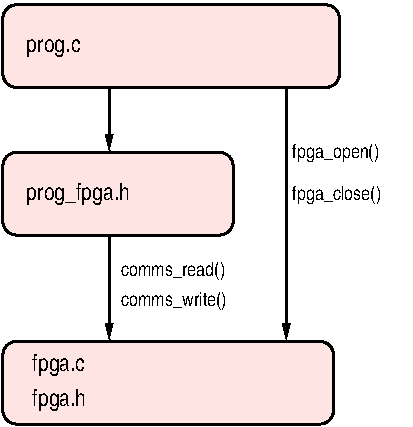
\includegraphics{c_zynq}
        
        For details see (\autorefph{ch:tools_c_zynq}).

        The following C program includes the above file. Note that in the case of
        a Python3 program the interface information can be read from the FPGA and
        compiled as a module If the interface information has been incorporated
        into block RAM in the FPGA. This cannot be done with a C interface and
        thus directive "excludeinfo" should be set true to avoid wasting these
        logic and memory resources;
        
        \begin{lstlisting}[gobble=4, language=C]
            #include <stdio.h>
            #include <stdlib.h>
            #include <stdint.h>
            #include <pthread.h>
            #include "/root/install/3pl/fpga.h"

            int64_t     p;

            void*       INT_handler ();
            pthread_t   thread_start(
                            void *  (*func)(void*),
                            void *  arg,
                            char *  name,
                            int     priority
                        );

            #include    "prog_cinclude.h"

            #include    "prog_fpga.h"

            int
            main (
                int     argc,
                char**  argv
            ) {    
                pthread_t   INT_thread;
                int         pri_min = 1;

                // Open the CPU interface.
                fpga_open();

                // Load the configuration.
                //fpga_configdata_load(prog_fpga_config_data, prog_fpga_config_size);
                fpga_configfile_load("prog.bit");

                // Start a thread for the interrupt
                INT_thread  = thread_start(INT_handler,  NULL, "INT_handler",  pri_min);

                fpga_A_write(123);
                fpga_B_write(1);
                p = fpga_P_read();
                printf("read %lld (should be 123)\n", p);
                fpga_A_write(1);   // will generate an interrupt
                sleep(2);          // wait for the interrupt
                fpga_B_write(2);
                fpga_B_write(1);   // will generate another interrupt

                // Terminate the interrupt thread.
                pthread_cancel(INT_thread);


                // Close the CPU interface.
                fpga_close();

                exit(0);
            }

            void*
            INT_handler () {
                for(;;) {
                    fpga_INT_enable();
                    fpga_INT_wait();
                    printf("interrupt INT, p = %lld\n", p);
                    printf("number of events %d\n", fpga_INT_count());
                }
            }


            // Start a thread.
            pthread_t
            thread_start(
                void *  (*func)(void*),
                void *  arg,
                char *  name,
                int     priority
            ) {
                int                 status;
                struct sched_param  sp;
                pthread_t           tid;

                if ((status = pthread_create(&tid, NULL, func, arg)) != 0) {
	            printf("thread_start(): pthread_create() failed thread '%s' (err = %s)\n",
	                name, strerror(status));
                    exit(1);
                }

                sp.sched_priority = priority;

                status = pthread_setschedparam(tid, SCHED_RR, &sp);
                if (status != 0) {
    	            printf("thread_start(): pthread_setschedparam() failed for thread '%s' (err = %s)\n",
	                name, strerror(status));
                    exit(1);
                }
                return(tid);
            }
        \end{lstlisting}

        Include file "fpga.h" defines the basic FPGA communication interface
        functions.
        
        Include file "prog\_fpga.h" is created by python script 'info2c' and contains
        function definitions for each FPGA read, write or interrupt (event).
        These in turn use the functions in fpga.h above.

        {\bf fpga\_open()} sets up the ARM memory mapping for the AXI buses and devices
        associated with interrupts (events).

        {\bf fpga\_configdata\_load()} loads the FPGA configuration.  In this example
        the compressed FPGA configuration is compiled into the CPU program and is
        included from the file {\bf prog\_cinclude.h}. That file has been created by
        running program {\bf bin2c} which takes the configuration file prog.bit
        compresses it and then converts it to an array of hexadecimal constants. The
        FPGA configuration can alternatively be loaded from a file by the CPU if
        desired by calling {\bf fpga\_configfile\_load()} instead.

        Bus interfaces are used by calling the appropriate subroutines defined in prog\_fpga.h,
        in this case {\bf fpga\_A\_write()}, {\bf fpga\_B\_write()} and {\bf
        fpga\_P\_read()}, the bus addresses having been subsumed into the subroutine
        definitions. These functions are defined in 'prog\_fpga.h'.
        
        The C program must be linked with object file 'fpga.o' which can be
        compiled from source file 'fpga.c' located in the 3PL source directory
        'sources/fpga\_platforms/zynq/fpga'.



    \section{Python interface}

    
        As described previously the configuration file can be loaded into the
        FPGA manually by {\bf \verb'cat prog.bit >/dev/xdevcfg'}. Alternatively
        the configuration file prog.bit or compressed configuration file
        prog.bit.gz  can be converted into a byte array in source code.
    
        The configuration data can be incorporated into the CPU application
        program by using the utility {\bf bin2py} (sources/fpga\_platforms/bin2py).This
        will create a source file {\bf prog\_config.py} which can be
        imported into the application program.
        The configuration data can then be loaded into the FPGA by the
        application program by calling {\bf fpga\_configdata\_load()} -
        \begin{lstlisting}[gobble=4, language=Python]
            fpga_configdata_load(config.data, len(config.data))
        \end{lstlisting}
        
        The configuration can also be loaded from the uncompressed or compressed
        bit file during execution of the application program by calling {\bf
        fpga\_configfile\_load()}-
        \begin{lstlisting}[gobble=4, language=Python]
            fpga_configfile_load("prog.bit.gz"))
        \end{lstlisting}
        or
        \begin{lstlisting}[gobble=4, language=Python]
            fpga_configfile_load("prog.bit"))
        \end{lstlisting}
        

        
        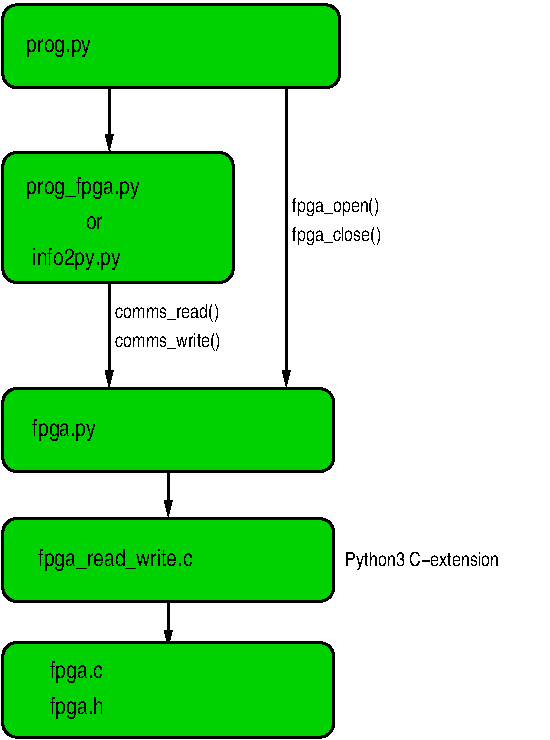
\includegraphics{py_zynq}
        
        For details see (\autorefph{ch:tools_python_zynq}).


    
        For a Python interface to the FPGA the modules {\bf info2py.py} (in
        directory fpga\_platforms/info2py) and functions in {\bf fpga.py} (in
        directory fpga\_platforms/zynq/fpga) must be imported.

        Functions in {\bf fpga.py} provide the code to open the interface to the
        FPGA, read and write to the FPGA and generate interrupts if required.

        info2py.py either reads the .info file (call info\_from\_file(file) or
        downloads the compressed info data in the FPGA (call info\_from\_fpga())
        and generates an internal module containing functions to access the FPGA
        register or memory interfaces.
        
        The 3PL module zynq\_axi.3pl will always produce a .info file. The
        compressed version loaded into block RAM in the FPGA configuration will
        be included by default but can be omitted by creating the directive
        "excludeinfo".
        
        The identifiers of the interface functions are listed in the report file,
        along with the data type. Each function is contained in the CPU\_API
        class {\bf fpga}.
    
        The previous 3PL source code can be used again as an example.

        The following Python source code would provide a CPU interface to the
        FPGA. The configuration file prog.bit is loaded into the FPGA by
        the application code by .
        
        The CPU/FPGA interface functions are defined
        in imported module {\bf prog\_fpga.py} which has been created by
        {\bf info2py prog}.
        
        {\bf fpga\_configfile\_load("prog.bit")}. This
        line could be omitted if the configuration was manually preloaded
        by executing {\bf cat prog.bit \verb'>'/dev/xdevcfg}.

        \begin{lstlisting}[gobble=4, language=Python]
            import sys
            import os
            sys.path.append(os.environ['HOME'] + "/install/3pl")
            from fpga import *
            import prog_fpga as fpga
            import time
            import signal
            import threading

            fpga_configfile_load("prog.bit")

            fpga_open()

            def INT_handler():
                while True:
                    fpga.INT_wait()
                    print("event INT")
                    print("number of events " + str(fpga.INT_count()))


            ev_INT = threading.Thread(target=INT_handler, args=(), daemon=True)
            ev_INT.start()

            a = 123
            b = 1

            fpga.A_write(a)
            fpga.B_write(b)
            print(str(fpga.P_read()) + "\t(should be 123)")
            a = 1
            fpga.A_write(a);    # will generate an interrupt
            a = 2
            fpga.A_write(a);
            a = 1
            fpga.A_write(a);    # will generate an interrupt

            time.sleep(1.0)     # wait for the interrupts

            fpga_close()

            os.kill(os.getpid(), signal.SIGTERM)    # use this to kill all threads!
        \end{lstlisting}

        As an alternative the configuration could be stored within the application
        code as an initialised byte array. Executing {\bf bin2py prog} will
        take prog.bit.gz and produce a Python3 module {\bf prog\_config.py}
        which can be imported to define the CPU/FPGA interface.


        \begin{lstlisting}[gobble=4, language=Python]
            import sys
            import os
            sys.path.append(os.environ['HOME'] + "/install/3pl")
            from fpga import *
            import prog_fpga as fpga
            import time
            import signal
            import threading
            import prog_config as config

            fpga_configdata_load(config.data, len(config.data))

            fpga_open()

            .
            .
            .

        \end{lstlisting}

        Instead of the CPU/FPGA interface definitions being imported
        from file {\bf prog\_fpga.py} as above they can be read from 
        {\bf prog.info} during execution using module {\bf info2py.py}.


        \begin{lstlisting}[gobble=4, language=Python]
            .
            .
            import info2py
            .
            .
            fpga_open()

            fpga = info2py.info_from_file("prog")   # load info from prog.info file
            .
            .
        \end{lstlisting}

        Another possibility is to import the CPU/FPGA interface definitions from
        the interface description embedded in the FPGA, assuming this has not
        been omitted by the directive "excludeinfo" true -


        \begin{lstlisting}[gobble=4, language=Python]
            .
            .
            import info2py
            .
            .
            fpga_open()

            fpga = info2py.info_from_fpga()         # load info from FPGA
            .
            .

        \end{lstlisting}
        
        The additional Python3 package path "/Users/..../install" depends on
        the layout of the file system, but the path component must contain
        "fpga.py" and "info2py".

        The Python3 library module {\bf fpga.py} must have been added by
        executing shell script {\bf mk\_setup} in {\bf ~/install/3pl/} on the
        Zynq CPU. This script runs setup.py which creates and adds the library
        module fpga\_py\_extension.c. Both {\bf setup.py} and {\bf mk\_setup} are installed in {\bf
        ~/install/3pl/setup.py}and the sources are in {\bf sources/tools/zynq}
        
        The Python CPU interface to the FPGA can read or write variables of any
        type to any degree of nesting, but there is a maximum variable size of 256
        bits (ldm/stm using 8 registers for a burst transfer). The following type
        conversions between 3PL and Python will occur -
         
        \begin{tabular}{| l | l | l |}
        \hline
        FPGA    & Python                \\
        \hline
        log     & logical               \\
        bits    & integer               \\
        uint    & integer               \\
        int     & integer               \\
        ufixed  & IEEE754 64bit float   \\
        fixed   & IEEE754 64bit float   \\
        float   & IEEE754 64bit float   \\
        struct  & dictionary            \\
        array   & list                  \\
        \hline
        \end{tabular}
        
        There are no run-time tests for data integrity, for example overflows.
        
        3PL arbitrary ufixed and fixed integer and fraction sizes are converted
        in or out of IEEE 64 bit floatin point in Python. Similarly 3PL arbitrary
        floating point biased exponent and mantissa sizes are again converted
        in or out of IEEE 64 bit floating point.
        
        A struct in 3PL is converted in or out of a dictionary in Python, the
        field name being the key.
        
        3PL multi-dimensional arrays are nested lists in Python.

    \section{An aside}

        As a matter of interest the following C function illustrates retrieval of the information string
        from the FPGA. The string length is returned as the function value and
        a pointer to the information string is assigned to the pointer argument.
        It is not necessary to use this function normally as the .info file can be
        converted to a C include file by using Python script 'info2c' as explained
        previously.

        \begin{lstlisting}[gobble=4, language=C]
           int fetch_info (unsigned char ** info) {
               int             i;
               int             n;
               int             e;
               unsigned long * buf;
               unsigned char * ubuf;
               unsigned long * bufp;
               unsigned long   ulen;

               fpga_reg_write(1, 0);
               n = fpga_reg_read(1);    // number of bytes of compressed data
               ulen = n * 10;           // enough room for uncompressed data (a guess)

               buf = malloc(n+3);       // enough room for compressed data, 32-bit packed
               ubuf = malloc(ulen);
               bufp = buf;
               for (i=0 ; i<n ; i+=4)
                   *bufp++ = fpga_reg_read(1);

               e = uncompress(ubuf, &ulen, ((Byte *)buf), n);
               if (e != Z_OK) {
                   printf("info uncompress error %d\n", e);
                   return(-1);
               }

               free(buf);
               *info = realloc(ubuf, ulen); // eliminate unused trailing buffer space
               return(ulen);
           }
        \end{lstlisting}
        
        But alas in C this interface information cannot be used, as it can in
        Python3.

        In the case of Python3, the following code would retrieve the JSON info
        from the FPGA data as a string -


        \begin{lstlisting}[gobble=4, language=Python]
            #----------------------------------------------------------------------
            # Read the compressed JSON structure from the FPGA
            # and expand it. Return a code module containing the interface
            # functions.
            #
            def info_from_fpga ():
                # reset the json interface
                fpga_rw.comms_write(0, 2, 0, None)

                # get the checksum
                rba = fpga_rw.comms_read(0, 1, 0, 4)
                checksum = int.from_bytes(rba, byteorder=bo, signed=False)

                # get the uncompressed byte count
                rba = fpga_rw.comms_read(0, 1, 0, 4)
                ucl = int.from_bytes(rba, byteorder=bo, signed=False)

                # get the compressed byte count
                rba = fpga_rw.comms_read(0, 1, 0, 4)
                cl = int.from_bytes(rba, byteorder=bo, signed=False)

                # read the compressed json info string
                words = cl // 4 + 1
                rba = bytearray()
                for i in range(words):
                    rba += fpga_rw.comms_read(0, 1, 0, 4)

                # decompress the json string
                infostring = zlib.decompress(rba[2:-4], -15)

                return(str(infostring, 'utf-8'))
        \end{lstlisting}


